\documentclass[a4paper]{article}
\usepackage[spanish]{babel}
\usepackage[utf8]{inputenc}
\usepackage{graphicx}
\usepackage{pdfpages}
\usepackage{enumerate}
\usepackage{listings}
\usepackage{color}
\usepackage{indentfirst}
\usepackage{fancyhdr}
\usepackage{latexsym}
\usepackage[colorlinks=true, linkcolor=black]{hyperref}
%\usepackage{makeidx}
%\usepackage{float}
\usepackage{wrapfig}
\usepackage{calc}
\usepackage{amsmath, amsthm, amssymb}
\usepackage{amsfonts}
%\lstset{language=C}
\definecolor{gray}{gray}{0.5}
\definecolor{light-gray}{gray}{0.95}
\definecolor{orange}{rgb}{1,0.5,0}

\usepackage{fancyhdr}
\pagestyle{fancy}

%\renewcommand{\chaptermark}[1]{\markboth{#1}{}}
\renewcommand{\sectionmark}[1]{\markright{\thesection\ - #1}}

\fancyhf{}

\fancyhead[LO]{Sección \rightmark} % \thesection\
\fancyfoot[LO]{\small{Raul Benitti, Damián Castro, Leandro Matayoshi, Javier San Miguel}}
\fancyfoot[RO]{\thepage}
\renewcommand{\headrulewidth}{0.5pt}
\renewcommand{\footrulewidth}{0.5pt}
\setlength{\hoffset}{-0.8in}
\setlength{\textwidth}{16cm}
%\setlength{\hoffset}{-1.1cm}
%\setlength{\textwidth}{16cm}
\setlength{\headsep}{0.5cm}
\setlength{\textheight}{25cm}
\setlength{\voffset}{-0.7in}
\setlength{\headwidth}{\textwidth}
\setlength{\headheight}{13.1pt}

\renewcommand{\baselinestretch}{1.1}  % line spacing


% \setcounter{secnumdepth}{2}
\usepackage{underscore}
\usepackage{caratula}
\usepackage{url}
\usepackage{float}
\usepackage[noend]{algpseudocode}

\newcommand{\cod}[1]{{\tt #1}}
\newcommand{\negro}[1]{{\bf #1}}
\newcommand{\ital}[1]{{\em #1}}
\newcommand{\may}[1]{{\sc #1}}
\newcommand{\tab}{\hspace*{2em}}

\hypersetup{
 pdfstartview= {FitH \hypercalcbp{\paperheight-\topmargin-1in-\headheight}},
 pdfauthor={Grupo},
 pdfsubject={Dise\~{n}o}
}

\lstdefinestyle{customc}{
  backgroundcolor=\color{light-gray},
  belowcaptionskip=1\baselineskip,
  breaklines=true,
  numbers=left,
  xleftmargin=\parindent,
  language=C,
  showstringspaces=false,
  basicstyle=\footnotesize\ttfamily,
  keywordstyle=\bfseries\color{blue},
  commentstyle=\itshape\color{gray},
  identifierstyle=\color{black},
  stringstyle=\color{orange},
}

\lstdefinestyle{customasm}{
  backgroundcolor=\color{light-gray},
  belowcaptionskip=1\baselineskip,
  numbers=left,
  xleftmargin=\parindent,
  language=[x86masm]Assembler,
  keywordstyle=\bfseries\color{blue},
  basicstyle=\footnotesize\ttfamily,
  commentstyle=\itshape\color{gray},
}

\lstset{escapechar=@}


\begin{document}

\thispagestyle{empty}
\materia{Bases de Datos}
\submateria{Segundo Cuatrimestre de 2015}
\titulo{Trabajo Práctico I}
%\subtitulo{Scheduling}
\integrante{Raul Benitti}{592/08}{raulbenitti@gmail.com }
\integrante{Damian Castro}{326/11}{ltdicai@gmail.com }
\integrante{Leandro Matayoshi}{79/11}{leandro.matayoshi@gmail.com }
\integrante{Javier San Miguel}{786/10}{javiersm00@gmail.com}

\makeatletter

\maketitle
\newpage

\thispagestyle{empty}
\vfill

\thispagestyle{empty}
\vspace{3cm}
%\tableofcontents
\newpage

\newenvironment{myindentpar}[1]
{\begin{list}{1}
         {\setlength{\leftmargin}{#1}}
         \item[]
}
{\end{list} }

%\normalsize
\newpage

% -------------------------------------------------------
% DER
% -------------------------------------------------------
\section{Introduccion}

El objetivo del trabajo es modelar, dise\~nar e implementar la base de datos \textbf{\emph{RUAT}}
(Registro Único de Accidentes de Tránsito).

La misma consiste en un Sistema Nacional de Registro de Accidentes Viales. Tal como su nombre lo indica, el mayor interés
está enfocado en la posibilidad de efectuar consultas respecto a los accidentes de tránsito acaecidos. Quiénes son los
conductores de los vehículos causantes de los accidentes, en qué lugares se produjeron, quiénes son los testigos,
número de patente de los vehículos, etc., son ejemplos de datos importantes
que se desea conocer y por los que se quiere buscar.

Además de llevar un registro de accidentes, se desea incorporar como información adicional los datos relacionados con
infracciones de tránsito y antecedentes penales de las personas involucradas en los siniestros.

Por último, se quiere contar también con información del parque automotor que circula por el país: compa\~nía de seguros,
categoría, antigüedad, cobertura de cada vehículo, etc.

\subsection{Motor de base de datos}

El motor de base de datos elegido fue SQL Server porque fue el utilizado por la cátedra durante el laboratorio de datos
de bases de datos relacionales. Además está instalado en las máquinas del laboratorio, lo cual facilita la demostración
presencial. De cualquier manera, consideramos que no hubiera sido muy diferente realizar otra elección, ya que los otros
motores: \textbf{\underline MySQL}, \textbf{\underline SQLite} se asemejan en cuanto a la sintaxis y funcionalidades a la
hora de implementar bases de datos estándar.
\newpage

En primer lugar realizamos un relevamiento de los requerimientos, lo cual nos permitió separar los objetivos del sistema en categorías generales. El paso posterior
fue dividir cada una de estar categorías principales en objetivos más peque\~nos. Este diagrama nos permite identificar las funcionalidades que debe tener nuestro 
sistema de manera resumida.

\begin{enumerate}
	\item{Mantener información general sobre las infracciones y los siniestros ocurridos en el sistema de tránsito:}
		\begin{enumerate}
			\item Conductores
			\item Modalidad del siniestro
				\begin{enumerate}
					\item Atropello
					\item Vuelco
					\item Incendio
					\item Choque
				\end{enumerate}
		\end{enumerate}
	\item{Mantener información particular sobre los accidentes}
		\begin{enumerate}
			\item Mantener información sobre la fecha y hora del siniestro
			\item Mantener información sobre la ubicación del siniestro
			\item{Mantener información sobre las personas involucradas en el siniestro. Diferenciar roles de las mismas en relación al accidente:}
				\begin{enumerate}
					\item Conductor
					\item Acompa\~nante
					\item Tercero accidentado
					\item Testigo
				\end{enumerate}
			\item Mantener información sobre la denuncia policial
				\begin{enumerate}
					\item Fecha de la denuncia
					\item Comisaría en donde se realizó la denuncia
					\item Oficial que elevó la denuncia
				\end{enumerate}
			\item Mantener información sobre los peritajes
				\begin{enumerate}
					\item Información general del reporte
						\begin{enumerate}
							\item Fecha
							\item Perito responsable
						\end{enumerate}
					\item Motivo del peritaje
						\begin{enumerate}
							\item Causa probable o presunta del accidente
							\item Sobre qué pavimento se produjo
							\item ¿Las víctimas usaban cinturón?
							\item Estado y condiciones de la vía
							\item Estado de iluminación
							\item Condiciones climáticas
							\item ¿Se contaba con elementos de seguridad?
						\end{enumerate}
				\end{enumerate}
		\end{enumerate}
	\item{Mantener información general sobre los lugares}
		\begin{enumerate}
			\item Tipo de lugar
				\begin{enumerate}
					\item Ruta
						\begin{enumerate}
							\item Nacional
							\item Provincial
						\end{enumerate}
					\item Calle
						\begin{enumerate}
							\item Provincia
							\item Ciudad
						\end{enumerate}
				\end{enumerate}	
			\item Tipo de asfalto
				\begin{enumerate}
					\item Asfalto
					\item Cemento
					\item Ripio
					\item Tierra
				\end{enumerate}
			\item Longitud
			\item Nombre
			\item Velocidad máxima permitida
		\end{enumerate}
	\item{Mantener información sobre el parque automotor}
		\begin{enumerate}
			\item Modelo
			\item Antigüedad
			\item Aseguradora
			\item Tipo de cobertura
			\item Categoría 
				\begin{enumerate}
					\item Alta
					\item Media
					\item Baja
				\end{enumerate}
			\item{Utilitario}
			\item Conductores habilitados
		\end{enumerate}
	\item{Mantener información general sobre los conductores}
		\item Información de la Licencia
			\begin{enumerate}
				\item Fecha de otorgamiento
				\item Fecha de caducidad
				\item Para qué tipo de vehículo
			\end{enumerate}
		\item DNI de los conductores
\end{enumerate}
\newpage

\section{Diagrama de Entidad Relación}

\begin{figure}
  \begin{center}
    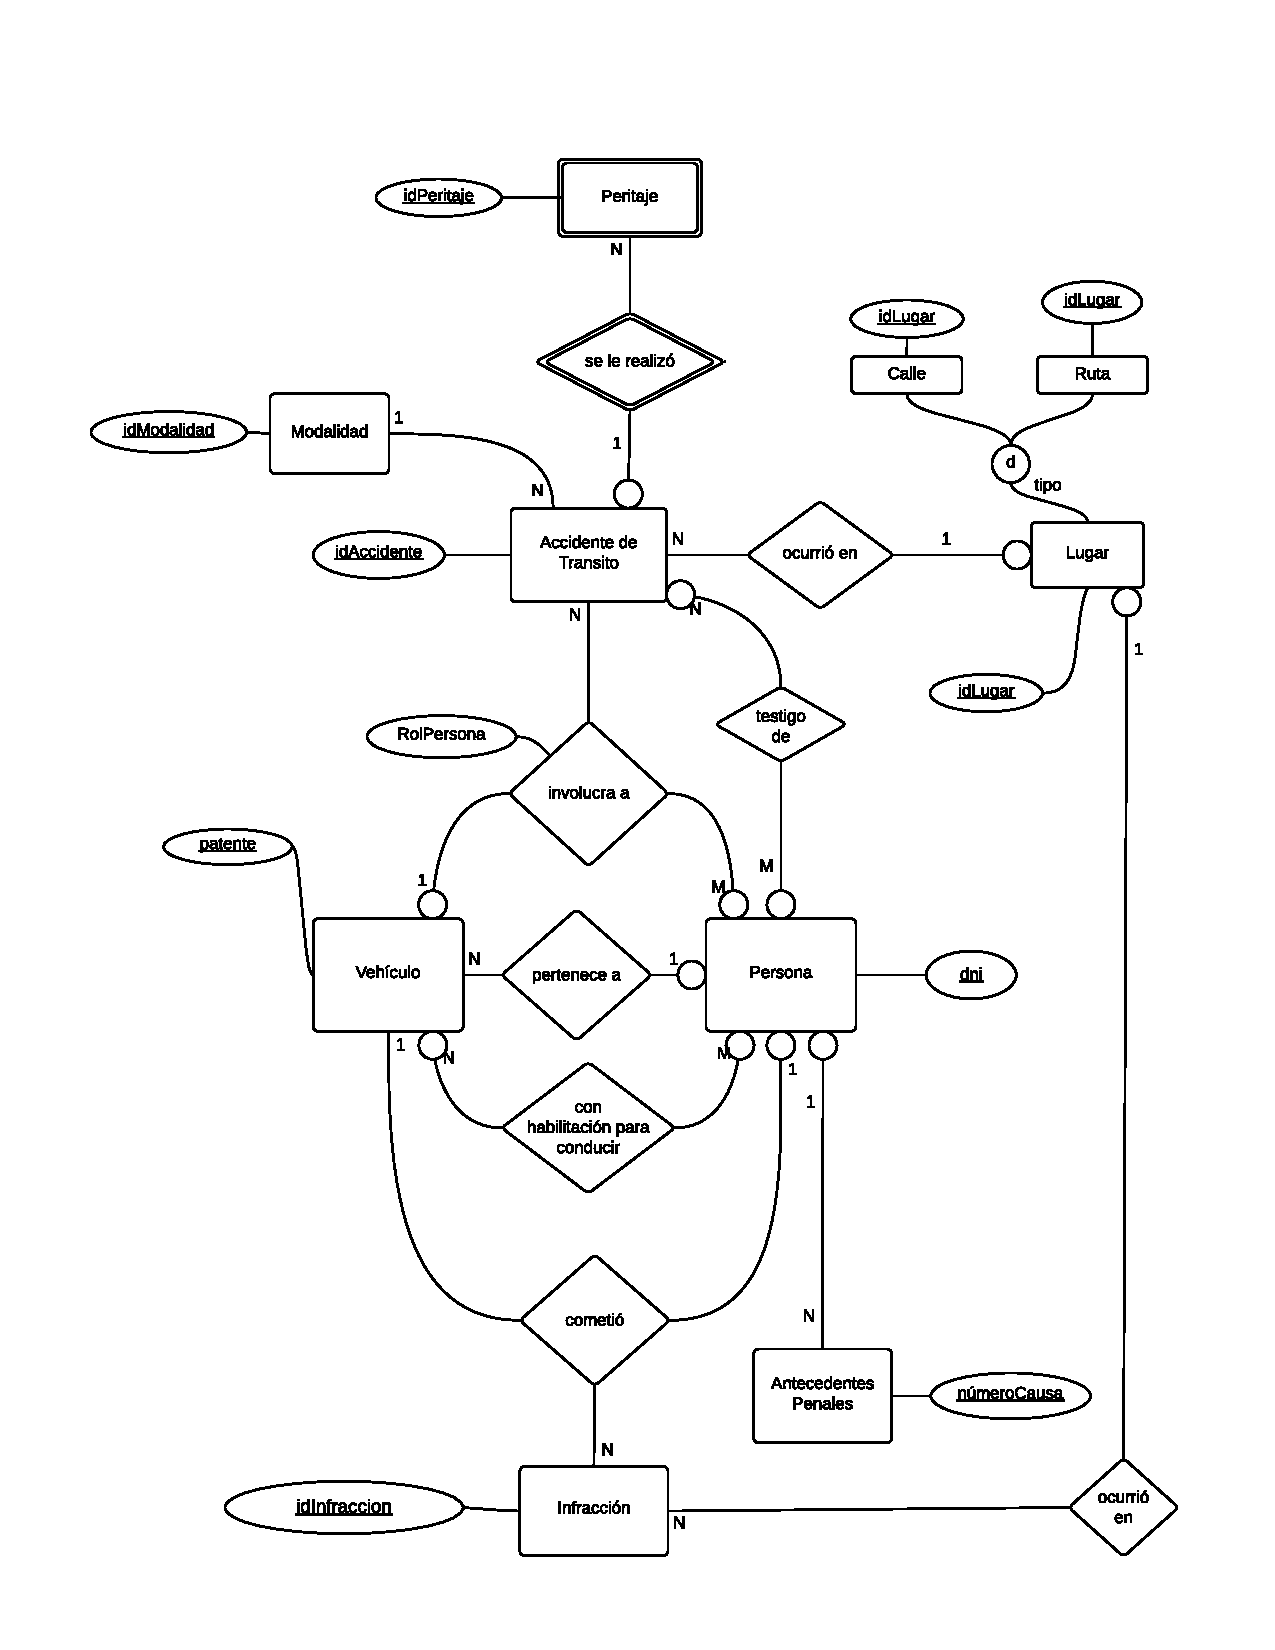
\includegraphics[scale=0.70]{diagramas/1.pdf}
    \caption{DER con PK's únicamente}
  \end{center}
\end{figure}

\subsection{Asunciones del dominio}

\begin{itemize}
  \item \textbf{DNI:} Todas las personas tienen DNI, y este es único para cada persona.
  \item \textbf{Lugar:} Los accidentes solo ocurren en calles y rutas. Por lo tanto se dividen en estas categorías(disjuntas).
  \item \textbf{Lugar:}  El tipo de pavimento de un lugar(calle o ruta) es uniforme a lo largo de toda su extensión.
  \item \textbf{Lugar:}  El tipo de pavimento de un lugar(calle o ruta) es uniforme a lo largo de toda su extensión. Es decir, no hay calles que estén asfaltadas en algunos tramos y no lo estén en otros.
  \item \textbf{Lugar:}  La velocidad máxima permitida de un lugar(calle o ruta) es uniforme a lo largo de toda su extensión.
  \item \textbf{Denuncias:}  Las denuncias policiales son tomadas por un único oficial.
  \item \textbf{Peritaje:}  Cada peritaje es realizado por un único perito.
  \item \textbf{Peritaje:}   Un peritaje consiste de un análisis de un factor relevante en el accidente. Por ejemplo, estado de iluminación de la vía al momento del accidente.
  \item \textbf{Peritaje:}  Cada peritaje tiene su resultado.
  \item \textbf{Accidente:}  Las personas tienen un único rol en un accidente: Pueden ser conductores o acompañantes de un vehículo, terceros afectados por este último o testigos. Los testigos no se relacionan con un vehículo en particular.
\end{itemize}

\subsection{DER con Primary Keys únicamente}
Como el diagrama está compuesto por muchas entidades con muchas relaciones, incluímos como primera aproximación un esqueleto
del modelo, en donde incluímos únicamente las entidades con sus claves primarias, la cardinalidad de las relaciones y
los atributos más relevantes.

\subsection{DER completo}
El diagrama completo fue separado en varias partes para facilitar su lectura.

\newpage
\begin{figure}
  \begin{center}
    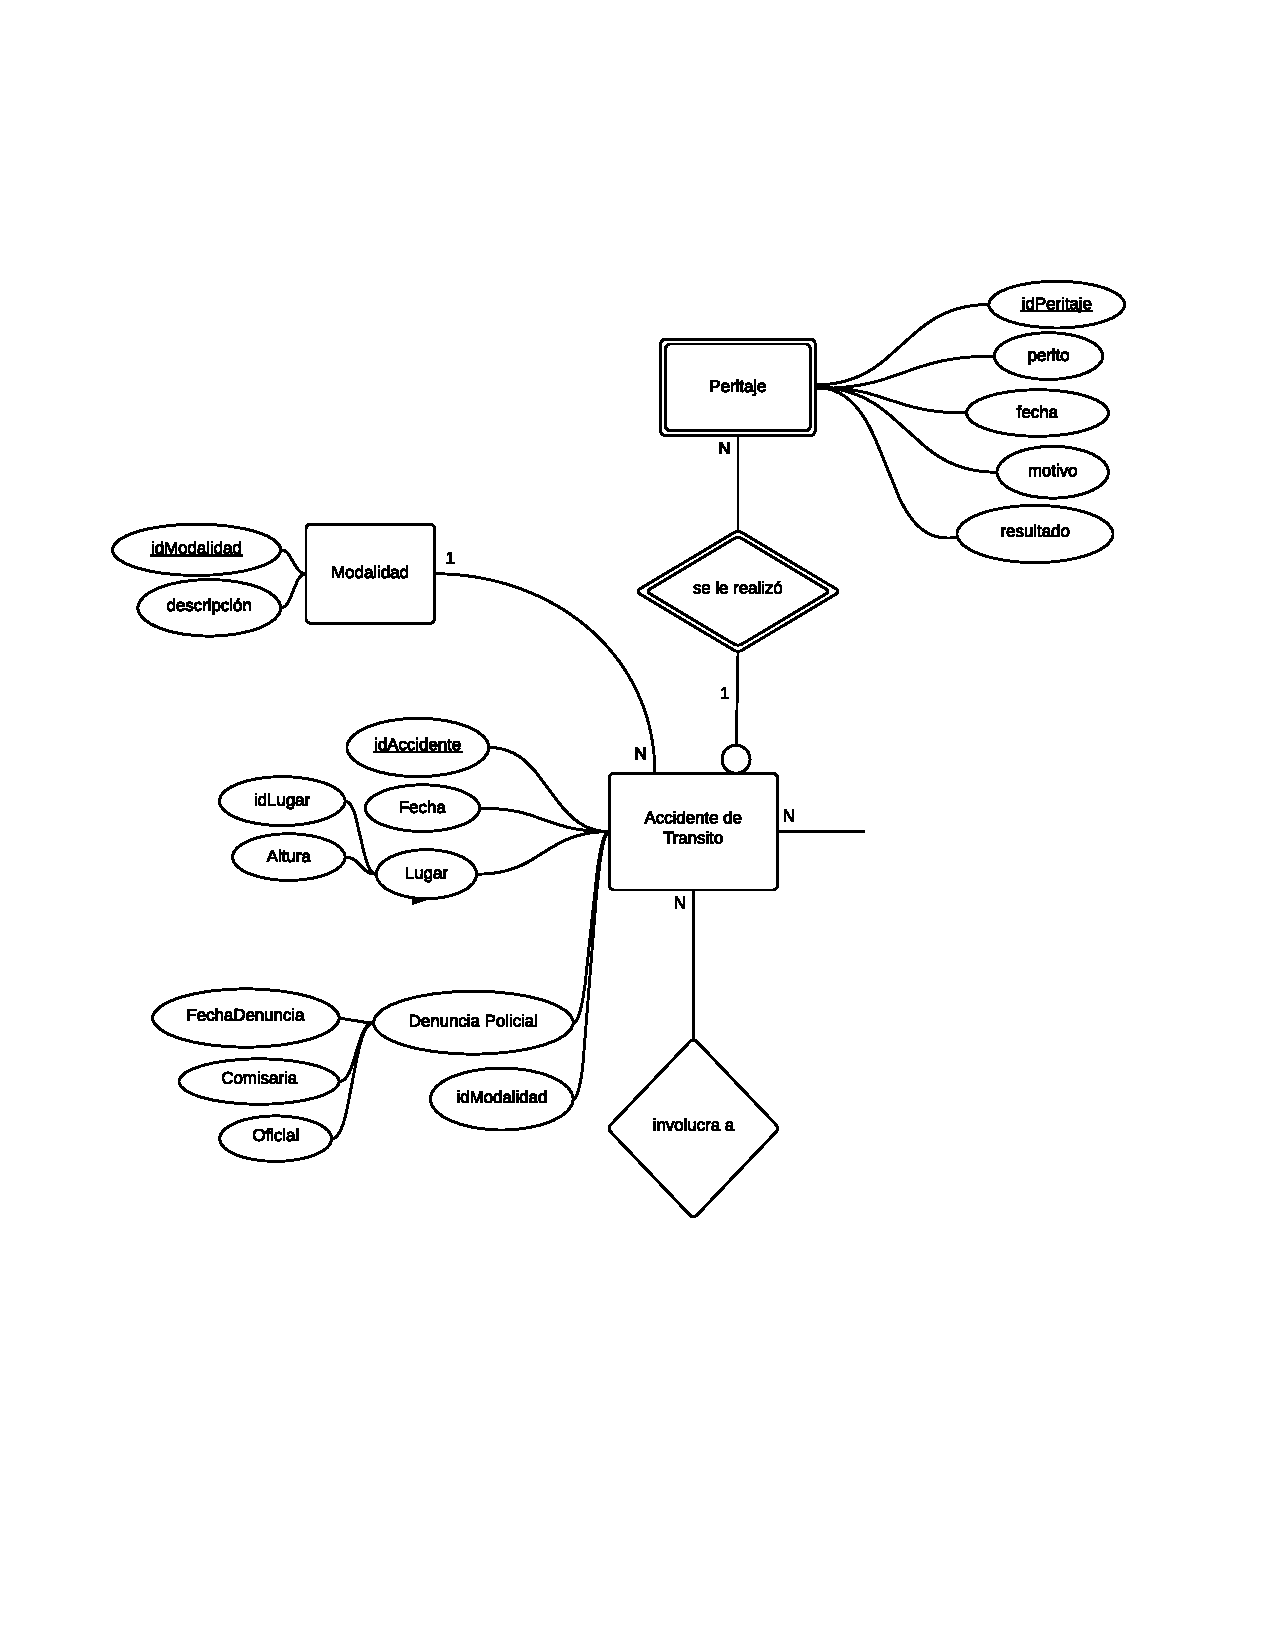
\includegraphics[scale=0.80]{diagramas/2-1.pdf}
    \caption{Accidente.Modalidad.Peritaje}
  \end{center}
\end{figure}

\newpage
\begin{figure}
  \begin{center}
    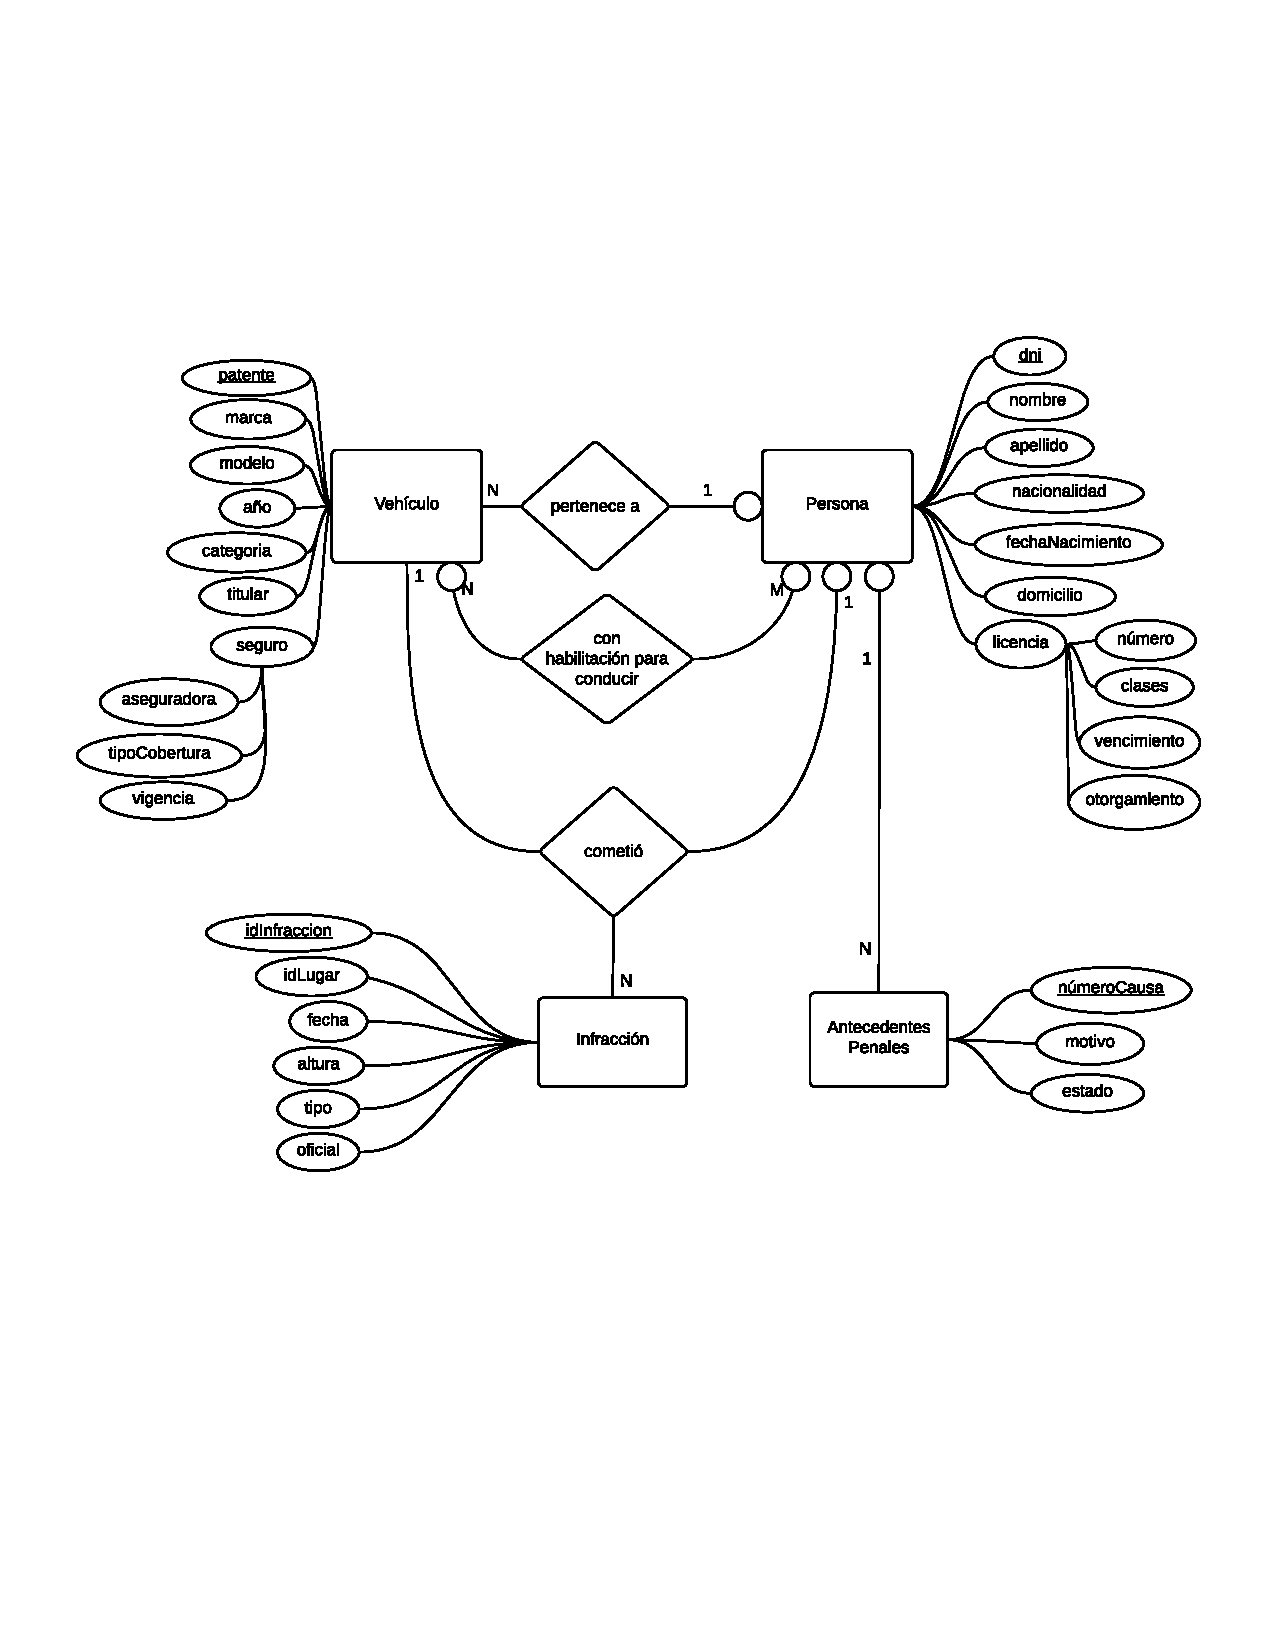
\includegraphics[scale=0.8]{diagramas/2-2.pdf}
    \caption{Vehículo.Persona.Antecedentes penales.Infracción}
  \end{center}
\end{figure}

\newpage
\begin{figure}
  \begin{center}
    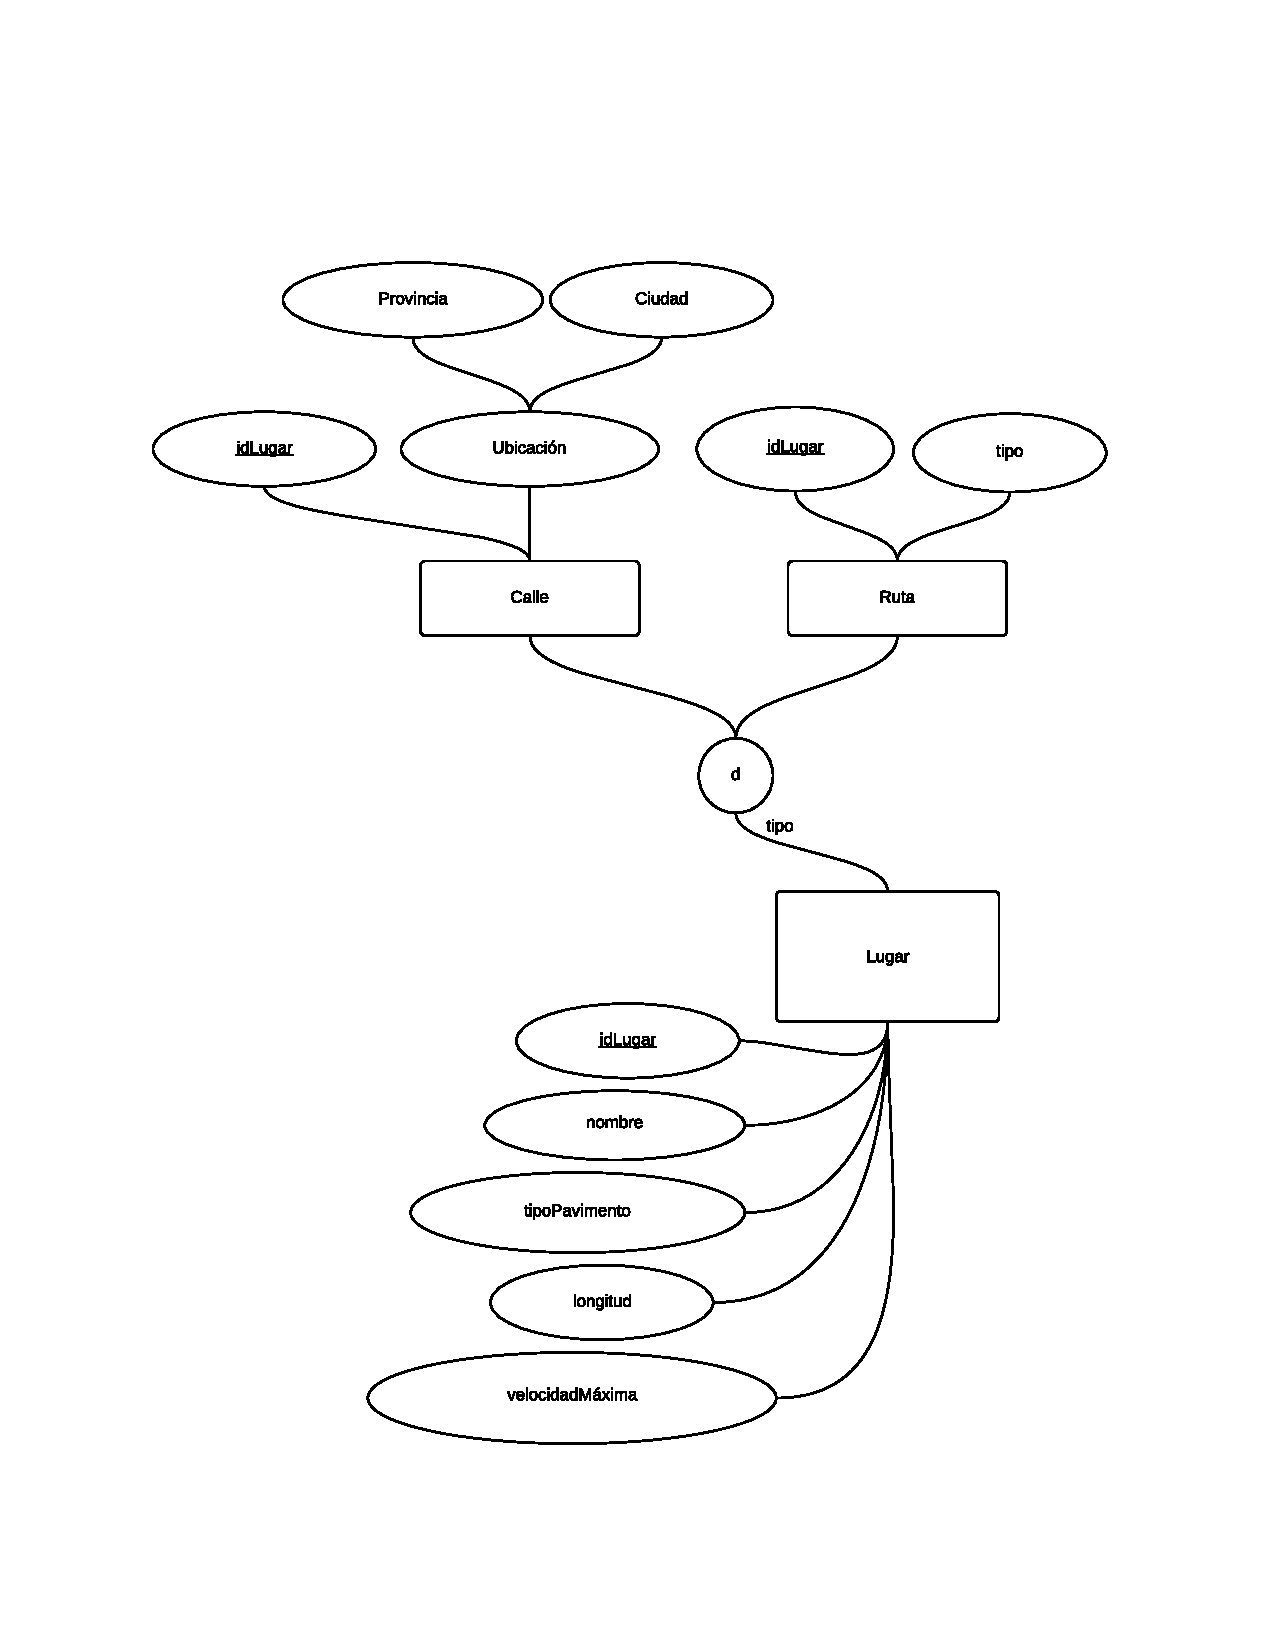
\includegraphics[scale=0.6]{diagramas/2-3.pdf}
    \caption{Lugar:Calle/Ruta}
  \end{center}
\end{figure}

\newpage
\begin{figure}
  \begin{center}
    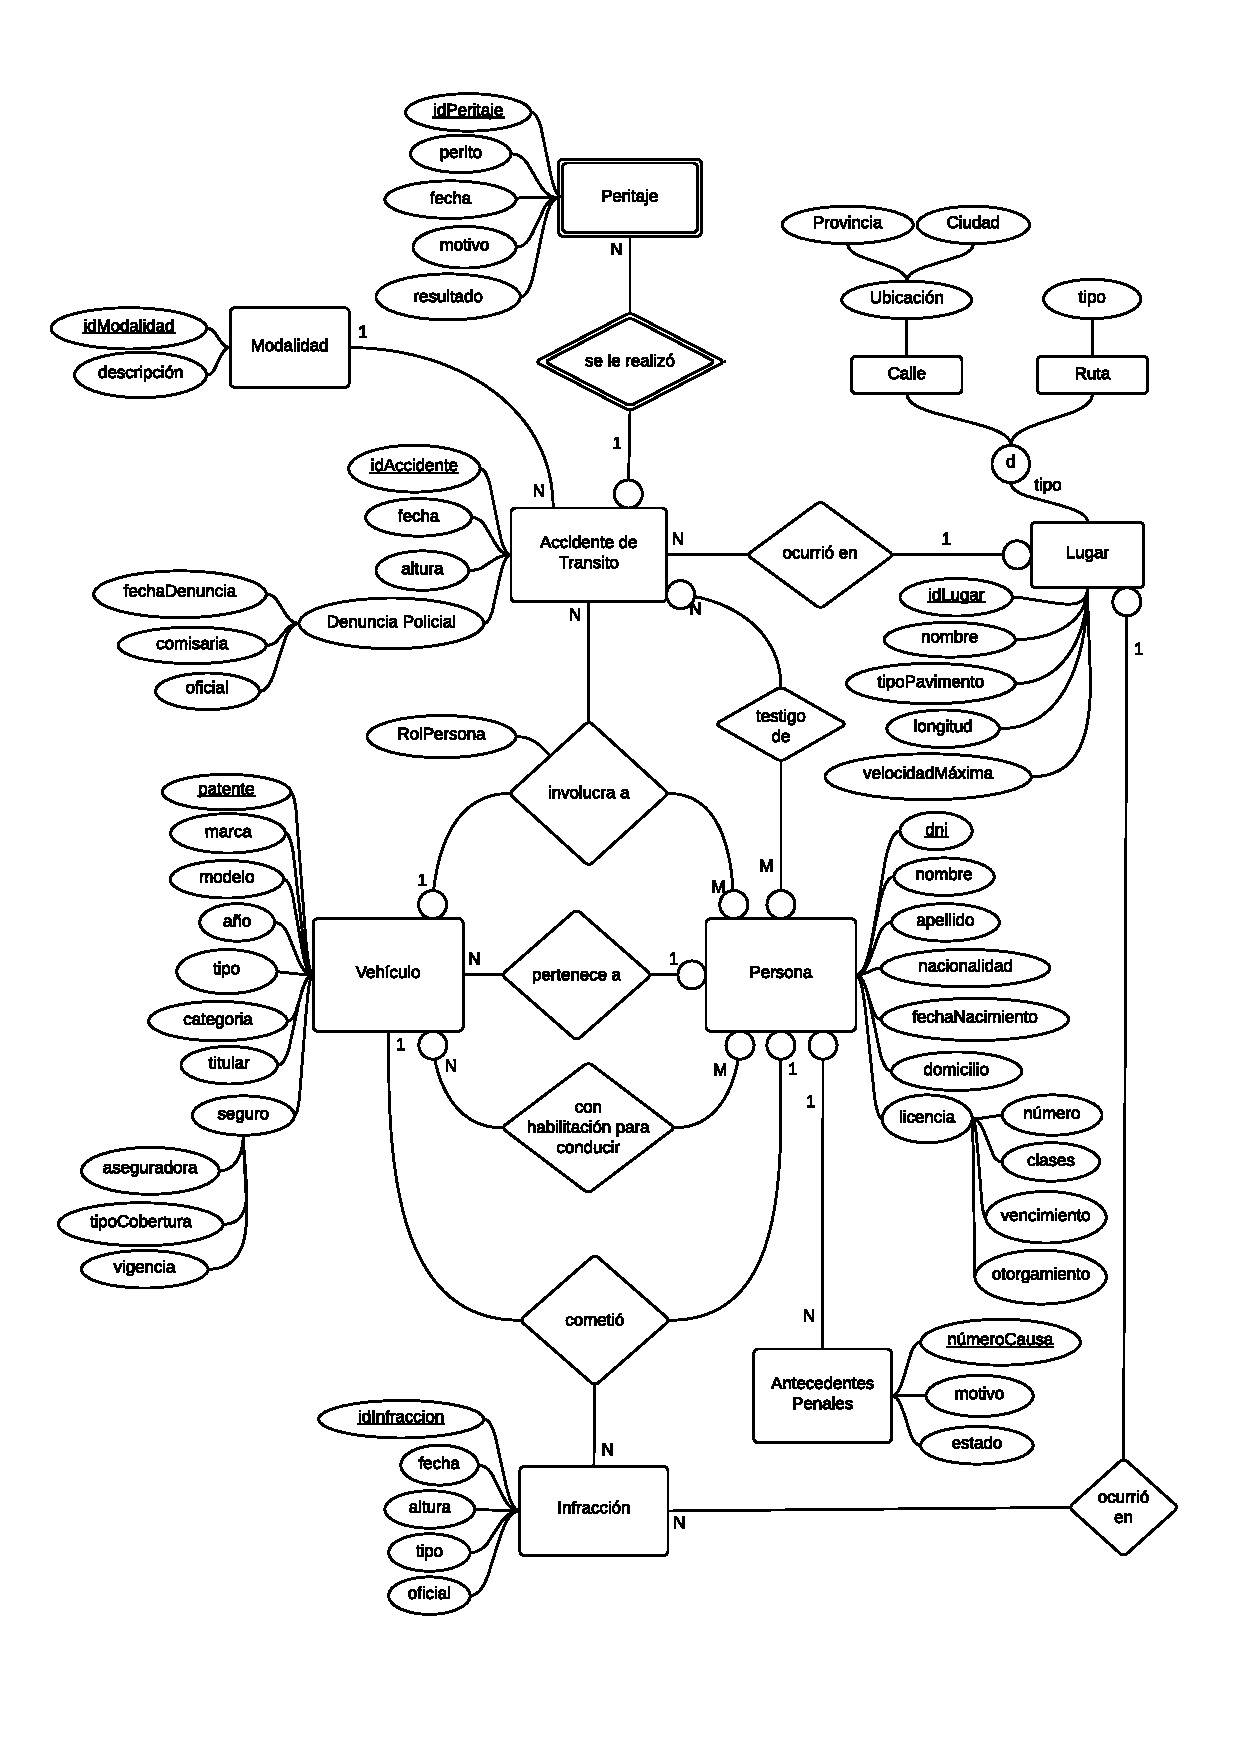
\includegraphics[scale=0.6]{diagramas/3.pdf}
    \caption{DER completo}
  \end{center}
\end{figure}


\newpage
\subsection{Reestricciones en lenguaje natural}

Cuestiones de notación: Cuando decimos que una entidad ''tiene'' un atributo, nos referimos a que dicho campo no puede ser \textbf{Null}.

\begin{enumerate}
  \item \textbf{Involucra_a:}
  \begin{enumerate}
    \item \textbf{Alguien manejaba y es único:} Dados un accidente y un vehículo involucrados en un accidente, existe una \underline{única} persona que manejaba ese vehículo en dicho accidente. Es decir, que tiene rol de conductor.
    \item \textbf{Conductores no son acompa\~nantes:} Las personas con rol de acompañante para un vehículo y un accidente no pueden estar involucrados como conductores de dicho vehículo en dicho accidente.
    \item \textbf{Conductores tienen licencia:} Las personas con rol de conductor de un vehículo en un accidente tienen licencia que les permite conducir ese vehículo.
    \item \textbf{Pasajeros no son testigos:} Las personas que están involucradas en un accidente y un vehículo no pueden ser testigos de los mismos.
    \item \textbf{Terceros afectados:} Los terceros afectados por un vehículo en un accidente no pueden ser conductores ni acompañantes en el mismo accidente.
    \item \textbf{Conductores tienen habilitación para conducir:} Si una persona conducía el vehículo en una accidente, entonces tiene habilitación para conducir ese vehículo.
  \end{enumerate}
  \item \textbf{Vehículo:}
    \begin{enumerate}
      \item \textbf{Tienen patente:} Todos los vehículos tienen patente, y ésta es única.
    \end{enumerate}
  \item \textbf{Peritaje:}
    \begin{enumerate}
      \item \textbf{Tienen motivo:} Los peritajes tienen descripción.
      \item \textbf{Tienen resultado:} Los peritajes tienen resultado.
      \item \textbf{Tienen fecha:} Los peritajes tienen fecha posterior a la del accidente.
      \item \textbf{Tienen perito:} Los peritajes son realizados por algún perito.
    \end{enumerate}
  \item \textbf{Denuncia:}
    \begin{enumerate}
      \item \textbf{Tienen denuncia:} Todos los accidentes tienen denuncia policial.
      \item \textbf{Denunciado en comisaría:} Las denuncias son hechas en una comisaría.
      \item \textbf{Realizada en una fecha específica:} Las denuncias son realizadas en una fecha. Ademàs, la fecha de la denuncia es igual o posterior a la fecha del accidente.
      \item \textbf{Acta labrada por un oficial:} El acta de las denuncias es labrada por un oficial.
    \end{enumerate}
\end{enumerate}






\newpage

\section{Modelo Relacional}

\begin{itemize}

\item Lugar(\underline{idLugar}, nombre, tipoPavimento, longitud, velocidaMaxima, tipo)
  \begin{itemize}
  \item[] PK = CK = \{idLugar\}
  \end{itemize}


\item Calle(\underline{idLugar}, provincia, ciudad)
  \begin{itemize}
  \item[] PK = CK = FK =\{idLugar\}
  \end{itemize}


\item Ruta(\underline{idLugar}, esNacional)
  \begin{itemize}
  \item[] PK = CK = FK =\{idLugar\}
  \end{itemize}


\item Persona(\underline{dni}, nombre, apellido, nacionalidad, fechaNacimiento, domicilio, numeroLic, clases, vencimiento, otorgamiento)
  \begin{itemize}
  \item[] PK = \{dni\}
  \item[] CK = \{dni, numeroLic\}
  \end{itemize}


\item Vehiculo(\underline{patente}, anio, tipo, marca, modelo, categoria, titular, aseguradora, tipoCobertura, vigenciaSeguro)
\begin{itemize}
  \item[] PK = CK = \{patente\}
  \item[] FK = \{dniDuenio\}
  \end{itemize}


\item Modalidad(\underline{idModalidad}, descripcion)
  \begin{itemize}
  \item[] PK = CK = \{idModalidad\}
  \end{itemize}


\item Accidente(\underline{idAccidente}, fecha, idLugar, altura, fechaDenuncia, comisaria, oficial, idModalidad)
  \begin{itemize}
  \item[] PK = CK = \{idAccidente\}
  \item[] FK = \{idLugar, idModalidad\}
  \end{itemize}

\item Infraccion(\underline{idInfraccion}, fecha, idLugar, altura, tipo, oficial)
  \begin{itemize}
  \item[] PK = CK = \{idInfraccion\}
  \item[] FK = \{idLugar\}
  \end{itemize}

\item HabilitacionConduccion(\underline{dni} , patente)
  \begin{itemize}
  \item[] PK = CK = \{(dni, patente)\}
  \item[] FK = \{dni, patente\}
  \end{itemize}

\item Testigo(\underline{idAccidente}, dni)
  \begin{itemize}
  \item[] PK = CK = \{(idAccidente, dni)\}
  \item[] FK = \{idAccidente, dni\}
  \end{itemize}

\item InfraccionVehiculoPersona(\underline{idInfraccion}, \underline{dni}, patente)
  \begin{itemize}
  \item[] CK = \{(idInfraccion, dni), (idInfraccion, patente)\}
  \item[] PK = \{(idInfraccion, dni)\}
  \item[] FK = \{idInfraccion, dni, patente\}
  \end{itemize}

\item AccidenteVehiculoPersona(\underline{idAccidente}, \underline{dni}, patente, rolPersona)
  \begin{itemize}
  \item[] PK = \{(idAccidente, dni), (idAccidente, patente)\}
  \item[] PK = \{(idAccidente, dni)\}
  \item[] FK = \{idAccidente, dni, patente\}
  \end{itemize}


\item Peritaje(\underline{idPeritaje}, \underline{idAccidente}, perito, fecha, motivo, resultado)
  \begin{itemize}
  \item[] PK = CK = \{idPeritaje, idAccidente\}
  \item[] FK = \{idAccidente\}
  \end{itemize}

\end{itemize}
\newpage
% ------------------------------------------------------
% Restricciones en lenguaje natural
% -------------------------------------------------------
\input{restricciones.tex}
\newpage
% ------------------------------------------------------
% queries y triggers
% -------------------------------------------------------
\footnotesize{
\begin{verbatim}
CREATE TABLE Lugar
(
    idLugar         int NOT NULL,
	nombre          varchar(128),
	tipoPavimento   varchar(256), 
	longitud        int, 
	velocidaMaxima  int,
	tipo            varchar(16) NOT NULL,
	PRIMARY KEY (idLugar)
);
Go

CREATE TRIGGER chkTipoLugar ON Lugar
FOR INSERT, UPDATE
AS 
BEGIN
    SET NOCOUNT ON;
    IF EXISTS (select 1 from inserted where tipo not in ('ruta', 'calle'))
        Rollback Transaction
END
Go

CREATE TABLE Calle
(
    idLugar 	int,
    provincia	varchar(128),
	ciudad		varchar(128),
	PRIMARY KEY (idLugar),
	FOREIGN KEY (idLugar) REFERENCES Lugar(idLugar)
);

CREATE TABLE Ruta
(
    idLugar 		int, 
    tipo            char(10),
	PRIMARY KEY (idLugar),
	FOREIGN KEY (idLugar) REFERENCES Lugar(idLugar)
);
Go
CREATE TRIGGER chkTipoRuta ON Ruta
FOR INSERT, UPDATE
AS 
BEGIN
    SET NOCOUNT ON;
    IF EXISTS (select 1 from inserted where tipo not in ('provincial', 'nacional'))
        Rollback Transaction
END
Go


CREATE TABLE Persona
(
    dni             int,
	nombre          varchar(128), 
	apellido        varchar(128), 
	nacionalidad    varchar(128), 
	fechaNacimiento datetime, 
	domicilio       varchar(256),
	numeroLic       int, 
    clasesLic       varchar(256),
    otorgamientoLic datetime, 
    vencimientoLic     datetime,
    PRIMARY KEY (dni)
);


CREATE TABLE Vehiculo
(
    patente   	    CHAR(6),
    marca           VARCHAR(48), 
    modelo          VARCHAR(48), 
	anio			smallint,
	tipo            varchar(16),
	categoria	    varchar(128),
	titular 		int,
	aseguradora		varchar(128),
	tipoCobertura	varchar(128),
	vigenciaSeguro  datetime, 		
	PRIMARY KEY (patente),
	FOREIGN KEY (titular) REFERENCES Persona(dni) 
);
GO
CREATE TRIGGER chkTipoVehiculo ON Vehiculo
FOR INSERT, UPDATE
AS 
BEGIN
    SET NOCOUNT ON;
    IF EXISTS (select 1 from inserted where tipo not in ('automovil', 'camion', 'motocicleta', 'camioneta', 'utilitario'))
        Rollback Transaction
END
Go


CREATE TABLE Modalidad
(
    idModalidad  int,
    descripcion varchar(32),
    PRIMARY KEY (idModalidad)
);


CREATE TABLE Accidente
(
    idAccidente		int, 
	fecha			datetime, 
	idLugar			int,
	altura		 	int,
	fechaDenuncia	datetime,	 
	comisaria		varchar(256), 
	oficial			varchar(256),
	idModalidad     int,
	PRIMARY KEY (idAccidente), 
	FOREIGN KEY (idLugar) REFERENCES Lugar(idLugar),
	FOREIGN KEY (idModalidad) REFERENCES Modalidad(idModalidad)
);


CREATE TABLE Infraccion
(
    idInfraccion int,
    fecha	 	 datetime,
    idLugar		 int,
	altura		 int,
    tipo	     varchar(256),
	oficial		 varchar(256),
	PRIMARY KEY (idInfraccion), 
	FOREIGN KEY (idLugar) REFERENCES Lugar(idLugar)
);


CREATE TABLE HabilitacionConduccion
(
    dni			int,
    patente		CHAR(6), 
	PRIMARY KEY (dni, patente),
    FOREIGN KEY (dni) REFERENCES Persona (dni), 
	FOREIGN KEY (patente) REFERENCES Vehiculo (patente)
);


CREATE TABLE Testigo
(
    idAccidente int,
    dni 		int,
    PRIMARY KEY (idAccidente, dni),
    FOREIGN KEY (idAccidente) REFERENCES Accidente(idAccidente),
    FOREIGN KEY (dni) REFERENCES Persona (dni)
);

CREATE TABLE InfraccionVehiculoPersona
(
    idInfraccion    int,
    dni             int,
    patente         CHAR(6),
    PRIMARY KEY (idInfraccion, dni),
    FOREIGN KEY (idInfraccion) REFERENCES Infraccion(idInfraccion),
    FOREIGN KEY (patente) REFERENCES Vehiculo (patente),
    FOREIGN KEY (dni) REFERENCES Persona (dni)
);

CREATE TABLE AccidenteVehiculoPersona
(
    idAccidente int,
    dni			int,
    patente 	CHAR(6),
	rolPersona	varchar(128),
    PRIMARY KEY (idAccidente, dni),
    FOREIGN KEY (idAccidente) REFERENCES Accidente (idAccidente),
    FOREIGN KEY (patente) REFERENCES Vehiculo (patente),
    FOREIGN KEY (dni) REFERENCES Persona (dni)
);

CREATE TABLE Peritaje
(
    idPeritaje int, 
    idAccidente int,
	perito		varchar(128), 
	fecha		datetime, 
	motivo		varchar(512), 
	resultado	varchar(8000),
    PRIMARY KEY (idAccidente, idPeritaje),
    FOREIGN KEY (idAccidente) REFERENCES Accidente (idAccidente)
);

CREATE TABLE AntecedentePenal 
(
    numeroCausa     int,
    dni             int,
    motivo          varchar(256),
    estado          varchar(32),
    FOREIGN KEY (dni) REFERENCES Persona (dni)
)

INSERT INTO Lugar(  idLugar, nombre, tipoPavimento, longitud, velocidaMaxima, tipo ) 
VALUES (1,'Ruta N40', 'ripio', 4500000, 30, 'ruta')
INSERT INTO Lugar(  idLugar, nombre, tipoPavimento, longitud, velocidaMaxima, tipo ) 
VALUES (2,'Avenida 9 de Julio', 'asfalto', 3600, 60, 'calle')
INSERT INTO Lugar(  idLugar, nombre, tipoPavimento, longitud, velocidaMaxima, tipo ) 
VALUES (3,'Junin', 'asfalto', 4000, 40,'calle') 
INSERT INTO Lugar(  idLugar, nombre, tipoPavimento, longitud, velocidaMaxima, tipo ) 
VALUES (4,'Avenida 9 de Julio', 'asfalto', 1900, 40,'calle')
INSERT INTO Lugar(  idLugar, nombre, tipoPavimento, longitud, velocidaMaxima, tipo ) 
VALUES (5,'Yapeyu', 'asfalto', 800, 40,'calle')
INSERT INTO Lugar(  idLugar, nombre, tipoPavimento, longitud, velocidaMaxima, tipo ) 
VALUES (6,'Ruta N4', 'asfalto', 4500, 30, 'ruta')
;
INSERT INTO Calle(  idLugar, provincia, ciudad ) VALUES (2, 'Capital Federal', 'Capital Federal')
INSERT INTO Calle(  idLugar, provincia, ciudad ) VALUES (3, 'Cordoba','Villa Carlos Paz')
INSERT INTO Calle(  idLugar, provincia, ciudad ) VALUES (4, 'Entre Rios', 'Chajari')
INSERT INTO Calle(  idLugar, provincia, ciudad ) VALUES (5, 'Capital Federal', 'Capital Federal')
;
INSERT INTO Ruta( idLugar, tipo ) VALUES (1, 'Nacional')
INSERT INTO Ruta( idLugar, tipo ) VALUES(6, 'Provincial')
;

INSERT INTO Persona( dni, nombre, apellido, nacionalidad, fechaNacimiento, domicilio,
 numeroLic,  clasesLic, otorgamientoLic, vencimientoLic) 
VALUES (24511187, 'Juan', 'Perez', 'argentino', '19480711', 'Riobamba 2323, CABA',11445123,
 'C, B2, D1', '20060701', '20160701')
INSERT INTO Persona( dni, nombre, apellido, nacionalidad, fechaNacimiento, domicilio,
 numeroLic,  clasesLic, otorgamientoLic, vencimientoLic) 
VALUES (95789111, 'Marco', 'Puertas', 'uruguayo', '19881221', 'Cochabamba 23, Santa Ana, Entre Rios', 
45632123, 'B1, C2', '20150501', '20250501')
INSERT INTO Persona( dni, nombre, apellido, nacionalidad, fechaNacimiento, domicilio,
 numeroLic,  clasesLic, otorgamientoLic, vencimientoLic) 
VALUES (34655298, 'Marta', 'Paredes', 'argentina', '19880908', '3 Arroyos 124, Ciudad Autonoma de Buenos Aires', 
24546788, 'B1', '20090101', '20190101')
INSERT INTO Persona( dni, nombre, apellido, nacionalidad, fechaNacimiento, domicilio,
 numeroLic,  clasesLic, otorgamientoLic, vencimientoLic) 
VALUES (54879213, 'Marcela', 'Morales', 'argentina', '19540321', 'San Martin 2344, Junin, Buenos Aires', 
24754575, 'A1, B1', '20110301', '20210301')
INSERT INTO Persona( dni, nombre, apellido, nacionalidad, fechaNacimiento, domicilio,
 numeroLic,  clasesLic, otorgamientoLic, vencimientoLic) 
VALUES (47111111, 'Emiliano', 'Rosales', 'argentino', '19430706', 'Venezuela 1789, Almagro, Capital Federal', 
19345677,  'B1', '20121201', '20221201')
GO
INSERT INTO Persona( dni, nombre, apellido, nacionalidad, fechaNacimiento, domicilio,
 numeroLic,  clasesLic, otorgamientoLic, vencimientoLic) 
VALUES (31849516, 'Rosario', 'San Marcos', 'argentina', '19841007', 'Gregoria Perez 3202, Capital Federal', 
30111345, 'A1', '20120301', '20220301')
GO
;

INSERT INTO Modalidad (idModalidad, descripcion) VALUES (1, 'atropello')
INSERT INTO Modalidad (idModalidad, descripcion) VALUES (2, 'vuelco')
INSERT INTO Modalidad (idModalidad, descripcion) VALUES (3, 'incendio')
INSERT INTO Modalidad (idModalidad, descripcion) VALUES (4, 'choque contra objeto estatito')
INSERT INTO Modalidad (idModalidad, descripcion) VALUES (5, 'caída del ocupante')
INSERT INTO Modalidad (idModalidad, descripcion) VALUES (6, 'choque en cadena')
INSERT INTO Modalidad (idModalidad, descripcion) VALUES (7, 'choque frontal')
;


INSERT INTO Vehiculo(  patente, marca, modelo, anio, tipo, categoria, titular ,aseguradora,
 tipoCobertura, vigenciaSeguro) 
VALUES ('CJK165', 'Peugeot', '306', 2006, 'automovil','sedan gama media', 24511187,  'La Caja',
 'Todo Total', '20160701' )
INSERT INTO Vehiculo(  patente, marca, modelo, anio, tipo, categoria, titular ,aseguradora,
 tipoCobertura, vigenciaSeguro) 
VALUES ('AAA456', 'Ford', 'Mondeo', 2006, 'automovil','sedan gama alta', 95789111,  'La Caja',
 'Terceros Completo con Granizo', '20160701' )
INSERT INTO Vehiculo(  patente, marca, modelo, anio, tipo, categoria, titular ,aseguradora,
 tipoCobertura, vigenciaSeguro) 
VALUES ('RWE951', 'Ford', 'F100', 1984, 'camioneta','gama media', 24511187,  'La Caja',
 'Responsabilidad Civil', '20160701' )
INSERT INTO Vehiculo(  patente, marca, modelo, anio, tipo, categoria, titular ,aseguradora,
 tipoCobertura, vigenciaSeguro) 
VALUES ('TKL111', 'Citroen', '3CV', 1972, 'automovil','sedan gama media', 34655298,  'La Caja',
 'Terceros Completo con Granizo', '20160701' )
INSERT INTO Vehiculo(  patente, marca, modelo, anio, tipo, categoria, titular ,aseguradora,
 tipoCobertura, vigenciaSeguro) 
VALUES ('EEE245', 'Toyota', 'Corola', 2010, 'automovil','sedan gama alta', 47111111,  'La Caja',
 'Responsabilidad Civil', '20160701' )
INSERT INTO Vehiculo(  patente, marca, modelo, anio, tipo, categoria, titular ,aseguradora,
 tipoCobertura, vigenciaSeguro) 
VALUES ('GHJ924', 'Ford', 'Taunus', 1973, 'batimovil','gama media', 47111111,  'La Caja',
 'Responsabilidad Civil', '20160701' )
;

INSERT INTO HabilitacionConduccion(  dni, patente ) VALUES (24511187, 'CJK165')
INSERT INTO HabilitacionConduccion(  dni, patente ) VALUES (95789111, 'AAA456')
INSERT INTO HabilitacionConduccion(  dni, patente ) VALUES (24511187, 'RWE951')
INSERT INTO HabilitacionConduccion(  dni, patente ) VALUES (34655298, 'TKL111')
INSERT INTO HabilitacionConduccion(  dni, patente ) VALUES (47111111, 'EEE245')
INSERT INTO HabilitacionConduccion(  dni, patente ) VALUES (24511187, 'EEE245')
INSERT INTO HabilitacionConduccion(  dni, patente ) VALUES (54879213, 'AAA456')
;


INSERT INTO Accidente(  idAccidente, fecha, idLugar, altura, fechaDenuncia,
 comisaria, oficial, idModalidad) 
VALUES (1,'20101005', 1, 2400, '20101005', 'Comisaria 123, San Rafael de Mendoza', 
'Teniente Juan Manuel Rosas', 2)
INSERT INTO Accidente(  idAccidente, fecha, idLugar, altura, fechaDenuncia,
 comisaria, oficial, idModalidad) 
VALUES (2,'20150417', 4, 1025, '20150418', 'Comisaria 15, Chajari', 'Pedro Moscano',7)
INSERT INTO Accidente(  idAccidente, fecha, idLugar, altura, fechaDenuncia,
 comisaria, oficial, idModalidad) 
VALUES (3,'20061224', 5, 493, '20061224', 'Comisaria 78, Almagro', 'Cabo Fernando Freitas', 1)
INSERT INTO Accidente(  idAccidente, fecha, idLugar, altura, fechaDenuncia,
 comisaria, oficial, idModalidad) 
VALUES (4,'20101005', 2, 3011, '20101005', 'Comisaria 123, San Rafael de Mendoza', 
'Teniente Juan Manuel Rosas',2)
INSERT INTO Accidente(  idAccidente, fecha, idLugar, altura, fechaDenuncia,
 comisaria, oficial, idModalidad) 
VALUES (5,'20121103', 2, 3011, '20121103', 'Comisaria 55, San Rafael de Mendoza', 'Jose Ramos',2)
INSERT INTO Accidente(  idAccidente, fecha, idLugar, altura, fechaDenuncia,
 comisaria, oficial, idModalidad) 
VALUES (6,'20140809', 3, 244, '20140809', 'Comisaria 74', 'Mariano Puentes' ,7)
;

INSERT INTO AccidenteVehiculoPersona(  idAccidente, dni, patente, rolPersona ) 
VALUES (1,24511187, 'RWE951', 'conductor')
INSERT INTO AccidenteVehiculoPersona(  idAccidente, dni, patente, rolPersona ) 
VALUES (2,24511187, 'CJK165', 'conductor')
INSERT INTO AccidenteVehiculoPersona(  idAccidente, dni, patente, rolPersona ) 
VALUES (2,34655298, 'TKL111', 'conductor')
INSERT INTO AccidenteVehiculoPersona(  idAccidente, dni, patente, rolPersona ) 
VALUES (3,24511187, 'CJK165', 'conductor')
INSERT INTO AccidenteVehiculoPersona(  idAccidente, dni, patente, rolPersona ) 
VALUES (3,34655298, 'CJK165', 'acompañante')
INSERT INTO AccidenteVehiculoPersona(  idAccidente, dni, patente, rolPersona ) 
VALUES (3,47111111, 'CJK165', 'atropellado')
INSERT INTO AccidenteVehiculoPersona(  idAccidente, dni, patente, rolPersona ) 
VALUES (4,47111111, 'EEE245', 'conductor')
INSERT INTO AccidenteVehiculoPersona(  idAccidente, dni, patente, rolPersona ) 
VALUES (4,95789111, 'EEE245', 'conductor')
INSERT INTO AccidenteVehiculoPersona(  idAccidente, dni, patente, rolPersona ) 
VALUES (5,24511187, 'RWE951', 'conductor')
INSERT INTO AccidenteVehiculoPersona(  idAccidente, dni, patente, rolPersona ) 
VALUES (6,34655298, 'TKL111', 'conductor')
INSERT INTO AccidenteVehiculoPersona(  idAccidente, dni, patente, rolPersona ) 
VALUES (6,24511187, 'TKL111', 'acompañante')
INSERT INTO AccidenteVehiculoPersona(  idAccidente, dni, patente, rolPersona ) 
VALUES (6,95789111, 'AAA456', 'conductor')
INSERT INTO AccidenteVehiculoPersona(  idAccidente, dni, patente, rolPersona ) 
VALUES (6,47111111, 'EEE245', 'conductor')
;

INSERT INTO Testigo(  idAccidente, dni ) VALUES (1,47111111 )
INSERT INTO Testigo(  idAccidente, dni ) VALUES (1,95789111 )
INSERT INTO Testigo(  idAccidente, dni ) VALUES (2,47111111 )
INSERT INTO Testigo(  idAccidente, dni ) VALUES (2,34655298 )
INSERT INTO Testigo(  idAccidente, dni ) VALUES (2,95789111 )
INSERT INTO Testigo(  idAccidente, dni ) VALUES (4,24511187 )
;

INSERT INTO Peritaje(  idPeritaje, idAccidente, perito, fecha, motivo, resultado ) 
VALUES (1, 1, 'Lic Jorge Garrafa', '20101006', 'Heridos', 'No se registraron.' )
INSERT INTO Peritaje(  idPeritaje, idAccidente, perito, fecha, motivo, resultado ) 
VALUES (2, 1, 'Lic Jorge Garrafa', '20101006', 'Uso de cinturon de seguridad', 
	'El conductor llevaba abrochado el cinturon de seguridad.' )
INSERT INTO Peritaje(  idPeritaje, idAccidente, perito, fecha, motivo, resultado ) 
VALUES (3, 1, 'Lic Jorge Garrafa', '20101006', 'Condiciones meteorologicas', 
	'Cielo despejado. Visibilidad normal a 1500m.' )
INSERT INTO Peritaje(  idPeritaje, idAccidente, perito, fecha, motivo, resultado ) 
VALUES (4, 1, 'Lic Jorge Garrafa', '20101006', 'Estado del asfalto', 
	'La ruta presentaba baches en la zona del accidente.' )
;

INSERT INTO Infraccion(  idInfraccion, fecha, idLugar, altura, tipo, oficial ) 
VALUES (1,'20010126', 2, 1234, 'Cruza semaforo en rojo', 'Martin Chomspy')
INSERT INTO Infraccion(  idInfraccion, fecha, idLugar, altura, tipo, oficial ) 
VALUES (2,'20010126', 3, 233, 'Estacionamiento no habilitado', 'Martin Chomspky')
INSERT INTO Infraccion(  idInfraccion, fecha, idLugar, altura, tipo, oficial ) 
VALUES (3,'20010126', 2, 756, 'Maxima velocidad superada', 'Marcelo Morela')
INSERT INTO Infraccion(  idInfraccion, fecha, idLugar, altura, tipo, oficial ) 
VALUES (4,'20010126', 1, 888, 'Cruza semaforo en rojo', 'Susana Trosky')
;

INSERT INTO InfraccionVehiculoPersona(  idInfraccion, dni, patente ) VALUES (1, 24511187,'RWE951')
INSERT INTO InfraccionVehiculoPersona(  idInfraccion, dni, patente ) VALUES (2, 54879213, 'AAA456')
INSERT INTO InfraccionVehiculoPersona(  idInfraccion, dni, patente ) VALUES (3, 24511187, 'CJK165')
INSERT INTO InfraccionVehiculoPersona(  idInfraccion, dni, patente ) VALUES (4, 47111111, 'EEE245')
;

INSERT INTO AntecedentePenal  (numeroCausa,dni,motivo,estado) 
VALUES (12332,24511187, 'Estafa', 'Sobreseido')
INSERT INTO AntecedentePenal  (numeroCausa,dni,motivo,estado) 
VALUES (12354,24511187, 'Defraudación', 'Sobreseido')
INSERT INTO AntecedentePenal  (numeroCausa,dni,motivo,estado) 
VALUES (75564,24511187, 'Amenazas', 'En tramite')
INSERT INTO AntecedentePenal  (numeroCausa,dni,motivo,estado) 
VALUES (32346,54879213, 'Usurpacion de autoridad', 'Sobreseido')
INSERT INTO AntecedentePenal  (numeroCausa,dni,motivo,estado) 
VALUES (97899,54879213, 'Tentativa de evasion impositiva', 'Procesado')
;
GO

SP: AccidentesPorLicencia
Parámetros: 
    licencia: int 
Devuelve los detalles de los accidentes en los que estuvo involucrada de alguna manera
la persona a la que corresponde la licencia parámetro.

IF EXISTS (SELECT 1 FROM sys.procedures where name = 'AccidentesPorLicencia')
    DROP PROCEDURE AccidentesPorLicencia
GO
CREATE PROCEDURE AccidentesPorLicencia @licencia int
AS
BEGIN
    SELECT  a.idAccidente, p.Nombre, p.Apellido, p.dni,  p.numeroLic as Licencia, avp.rolPersona as participacion, 
    m.descripcion, v.patente,  a.fecha, 
	CASE lu.tipo 
		WHEN 'ruta' THEN lu.nombre +' ('+ r.tipo +')'
		WHEN 'calle' THEN lu.nombre + ', '+ c.ciudad + ', '+ c.provincia
	END as 'lugar', a.altura,
	(select count(1) from HabilitacionConduccion WHERE dni = p.dni) as [Cantidad de autos habilitados]
    FROM AccidenteVehiculoPersona avp 
    INNER JOIN Persona p
    ON avp.dni = p.dni
    INNER JOIN Accidente a
    ON a.idAccidente = avp.idAccidente
    INNER JOIN Lugar lu
    ON lu.idLugar = a.idLugar
    INNER JOIN Modalidad m
    ON m.idModalidad = a.idModalidad
    INNER JOIN Vehiculo v
	ON v.patente = avp.patente
    LEFT JOIN Calle c
	on c.idLugar = lu.idLugar
	LEFT JOIN Ruta r
	on r.idLugar = lu.idLugar
	WHERE (@licencia is null or p.numeroLic = @licencia)
    order by a.idAccidente
    ;
END
GO

Vista: SumarioAccidentes
Cantidad de accidentes en los que participaron las personas cargadas en el 
sistema (identificadas por su licencia), agrupado por tipo de accidente.

IF EXISTS (SELECT 1 FROM sys.views where name = 'SumarioAccidentes')
    DROP VIEW SumarioAccidentes
GO
CREATE VIEW SumarioAccidentes AS
    select p.numeroLic as Licencia, m.descripcion as Modalidad, count(1) AS Cantidad
    from AccidenteVehiculoPersona avp
    INNER JOIN Accidente a
    ON a.idAccidente = avp.idAccidente
    INNER JOIN Modalidad m
    ON m.idModalidad = a.idModalidad
    INNER JOIN Persona p
    ON p.dni = avp.dni
    GROUP BY p.numeroLic, m.descripcion
GO

Debe mostrar los datos de los accidentes en los que participo el conductor con licencia 11445123

EXEC AccidentesPorLicencia 11445123
Go

Debe mostrar las licencia que participaron en choques frontales (junto con la cantidad de accidentes de tal 
tipo por cada licencia)

SELECT * FROM SumarioAccidentes where modalidad = 'choque frontal'
GO

Accidentes por tipo de vehiculo
Debe listar la cantidad de accidentes por tipo de vehiculo

SELECT v.tipo, COUNT(1) AS Cantidad
FROM AccidenteVehiculoPersona avp
INNER JOIN Vehiculo v
on v.patente = avp.patente
group by v.tipo

\end{verbatim}
}

\newpage
% ------------------------------------------------------
% conclusiones
% ------------------------------------------------------
\section{Conclusiones}

La base de datos obtenida satisface los requerimientos pautados por el enunciado. La implementación
es el resultado de un proceso que consta de 4 pasos:
\begin{itemize}
\item{Relevamiento de objetivos}
\item{Diagrama de entidad-relación}
\item{Modelo de entidad relación}
\item{Implementación}
\end{itemize}
Definir claramente los objetivos permitió abstraer el problema, transformándolo a un modelo de entidades y relaciones.
El DER es una herrmienta súmamente útil, ya que permite resumir la información de forma
visual y anticipar problemáticas que pueden llegar a surgir más adelante. La navegabilidad del diagrama determina
el alcance de las queries que quieran hacerse en el futuro.
El modelo de entidad relación es el paso intermedio entre el armado del diagrama y la implementación final.
Consideramos que la realización del trabajo práctico fue enriquecedor para nuestra formación, ya que nos permitió recorrer
por completo el proceso de creación de una base de datos relacional.


\bibliographystyle{plain}
\bibliography{tp3}

\end{document}
